%%%%%%%%%%%%%%%%%%%%%%%%%%%%%%%%%%%%%%%%%
% Arsclassica Article
% LaTeX Template
% Version 1.1 (10/6/14)
%
% This template has been downloaded from:
% http://www.LaTeXTemplates.com
%
% Original author:
% Lorenzo Pantieri (http://www.lorenzopantieri.net) with extensive modifications by:
% Vel (vel@latextemplates.com)
%
% License:
% CC BY-NC-SA 3.0 (http://creativecommons.org/licenses/by-nc-sa/3.0/)
%
%%%%%%%%%%%%%%%%%%%%%%%%%%%%%%%%%%%%%%%%%

%----------------------------------------------------------------------------------------
%	PACKAGES AND OTHER DOCUMENT CONFIGURATIONS
%----------------------------------------------------------------------------------------

\documentclass[
12pt, % Main document font size
a4paper, % Paper type, use 'letterpaper' for US Letter paper
oneside, % One page layout (no page indentation)
%twoside, % Two page layout (page indentation for binding and different headers)
headinclude,footinclude, % Extra spacing for the header and footer
BCOR5mm, % Binding correction
]{scrartcl}

%%%%%%%%%%%%%%%%%%%%%%%%%%%%%%%%%%%%%%%%%
% Arsclassica Article
% Structure Specification File
%
% This file has been downloaded from:
% http://www.LaTeXTemplates.com
%
% Original author:
% Lorenzo Pantieri (http://www.lorenzopantieri.net) with extensive modifications by:
% Vel (vel@latextemplates.com)
%
% License:
% CC BY-NC-SA 3.0 (http://creativecommons.org/licenses/by-nc-sa/3.0/)
%
%%%%%%%%%%%%%%%%%%%%%%%%%%%%%%%%%%%%%%%%%

%----------------------------------------------------------------------------------------
%	REQUIRED PACKAGES
%----------------------------------------------------------------------------------------

\usepackage[
nochapters, % Turn off chapters since this is an article        
beramono, % Use the Bera Mono font for monospaced text (\texttt)
eulermath,% Use the Euler font for mathematics
pdfspacing, % Makes use of pdftex’ letter spacing capabilities via the microtype package
dottedtoc % Dotted lines leading to the page numbers in the table of contents
]{classicthesis} % The layout is based on the Classic Thesis style

\usepackage{arsclassica} % Modifies the Classic Thesis package

\usepackage[T1]{fontenc} % Use 8-bit encoding that has 256 glyphs

\usepackage[utf8]{inputenc} % Required for including letters with accents

\usepackage{graphicx} % Required for including images
\graphicspath{{Figures/}} % Set the default folder for images

\usepackage{enumitem} % Required for manipulating the whitespace between and within lists

\usepackage{lipsum} % Used for inserting dummy 'Lorem ipsum' text into the template

\usepackage{subfig} % Required for creating figures with multiple parts (subfigures)

\usepackage{amsmath,amssymb,amsthm} % For including math equations, theorems, symbols, etc

\usepackage{varioref} % More descriptive referencing

%----------------------------------------------------------------------------------------
%	THEOREM STYLES
%---------------------------------------------------------------------------------------

\theoremstyle{definition} % Define theorem styles here based on the definition style (used for definitions and examples)
\newtheorem{definition}{Definition}

\theoremstyle{plain} % Define theorem styles here based on the plain style (used for theorems, lemmas, propositions)
\newtheorem{theorem}{Theorem}

\theoremstyle{remark} % Define theorem styles here based on the remark style (used for remarks and notes)

%----------------------------------------------------------------------------------------
%	HYPERLINKS
%---------------------------------------------------------------------------------------

\hypersetup{
%draft, % Uncomment to remove all links (useful for printing in black and white)
colorlinks=true, breaklinks=true, bookmarks=true,bookmarksnumbered,
urlcolor=webbrown, linkcolor=RoyalBlue, citecolor=webgreen, % Link colors
pdftitle={}, % PDF title
pdfauthor={\textcopyright}, % PDF Author
pdfsubject={}, % PDF Subject
pdfkeywords={}, % PDF Keywords
pdfcreator={pdfLaTeX}, % PDF Creator
pdfproducer={LaTeX with hyperref and ClassicThesis} % PDF producer
} % Include the structure.tex file which specified the document structure and layout

\usepackage{geometry}
\usepackage{float}

\hyphenation{Fortran hy-phen-ation e-ser-ci-ta-zio-ne} % Specify custom hyphenation points in words with dashes where you would like hyphenation to occur, or alternatively, don't put any dashes in a word to stop hyphenation altogether

%----------------------------------------------------------------------------------------
%	TITLE AND AUTHOR(S)
%----------------------------------------------------------------------------------------

\title{\normalfont\spacedallcaps{Relazione MEMOC}} % The article title

\author{\spacedlowsmallcaps{Giulio Lovisotto - 1084847} \\ \normalsize{\spacedallcaps{Universita' degli studi di Padova}}} % The article author(s) - author affiliations need to be specified in the AUTHOR AFFILIATIONS block

\date{16 Settembre 2015} % An optional date to appear under the author(s)

%----------------------------------------------------------------------------------------

\begin{document}

%----------------------------------------------------------------------------------------
%	HEADERS
%----------------------------------------------------------------------------------------

\renewcommand{\sectionmark}[1]{\markright{\spacedlowsmallcaps{#1}}} % The header for all pages (oneside) or for even pages (twoside)
%\renewcommand{\subsectionmark}[1]{\markright{\thesubsection~#1}} % Uncomment when using the twoside option - this modifies the header on odd pages
\lehead{\mbox{\llap{\small\thepage\kern1em\color{halfgray} \vline}\color{halfgray}\hspace{0.5em}\rightmark\hfil}} % The header style

\pagestyle{scrheadings} % Enable the headers specified in this block

%----------------------------------------------------------------------------------------
%	TABLE OF CONTENTS & LISTS OF FIGURES AND TABLES
%----------------------------------------------------------------------------------------

\maketitle % Print the title/author/date block

\setcounter{tocdepth}{2} % Set the depth of the table of contents to show sections and subsections only

%\tableofcontents % Print the table of contents

%\listoffigures % Print the list of figures

%\listoftables % Print the list of tables

%----------------------------------------------------------------------------------------
%	ABSTRACT
%----------------------------------------------------------------------------------------

%\section*{Abstract} % This section will not appear in the table of contents due to the star (\section*)

% \lipsum[1] % Dummy text

%----------------------------------------------------------------------------------------
%	AUTHOR AFFILIATIONS
%----------------------------------------------------------------------------------------

%{\let\thefootnote\relax\footnotetext{* \textit{Department of Biology, University of Examples, London, United Kingdom}}}

%{\let\thefootnote\relax\footnotetext{\textsuperscript{1} \textit{Department of Chemistry, University of Examples, London, United Kingdom}}}

%----------------------------------------------------------------------------------------

%\newpage % Start the article content on the second page, remove this if you have a longer abstract that goes onto the second page

%----------------------------------------------------------------------------------------
%	INTRODUCTION
%----------------------------------------------------------------------------------------

\section{Introduzione}

Questo documento descrive le metodologie e le strutture sviluppate per l'esercitazione del corso di Metodi e Modelli per l'Ottimizzazione combinatoria, anno accademico 14/15. L'esercitazione consiste nella risoluzione del  Traveling Salesman Problem (TSP) con l'uso di metodi di ottimizzazione. E' stato implementato il modello per il risolutore esatto \textsc{cplex}, e una metaeuristica di tipo particle swarm optimization \textsc{pso}. Il seguente documento e' strutturato come segue: in Sezione~\ref{sec:cplex} viene descritto il modello in \textsc{cplex} (relativo alla Parte 1), in Sezione~\ref{sec:eur} vengono descritte le euristiche utilizzate (relative allla Parte 2), in Sezione~\ref{sec:exp} vengono descritte le istanze del problema e la metodologia usata per l'esperimento, nonche' presentati i risultati. Il documento termina con alcune conclusioni in Sezione~\ref{sec:conclusioni}.

\subsection{FILES CONSEGNATI}

\begin{itemize}
\item something;
\item something else.
\end{itemize}

\section{Modello CPLEX} \label{sec:cplex}

In questa sezione viene descritto in che modo e' stato realizzato il modello per TSP che viene usato per la risoluzione con \textsc{cplex}. Per realizzare tale modello e' stata utilizzata la formalizzazione del TSP fornita dal docente~\cite{luigitraccia1}. Tale formalizzazione modella il problema come un problema di ottimizzazione su reti di flusso. E' stato realizzato un unico file \texttt{cplex.cpp}. Esso procede secondo i seguenti passi:
\begin{enumerate}
 \item legge il problema in input, che consiste in un file di testo riportante la matrice contenente i costi degli archi del grafo (separati da virgole), e inizializza le variabili del problema e la funzione obiettivo, impostando i vincoli di tipo e i bounds per ciascuna variabile;
 \item per ogni vincolo, lo crea e lo aggiunge alla matrice dei coefficienti dell'istanza del problema. Le variabili relative ai cappi (cioe' $x_{ii}, y_{ii}$) vengono rimosse;
 \item esegue l'ottimizzazione e salva i risultati su file, tra i quali tempo di esecuzione, path ottimo, costo della soluzione ottima trovata.
\end{enumerate}

%----------------------------------------------------------------------------------------
%	RESULTS AND DISCUSSION
%----------------------------------------------------------------------------------------

\section{Metaeuristiche} \label{sec:eur}
In questa sezione vengono descritte le metaeuristiche implementate per la risoluzione di TSP. 

\subsection{Particle Swarm Optimization}

\textsc{pso} e' una metaeuristica basata su popolazione. In esso, gli individui $x_k$ (possibili soluzioni) si muovono nello spazio N-dimensionale secondo le loro rispettive velocita' $v_k$. In \textsc{pso} gli individui ricordano la miglior posizione da loro visitata, e la miglior posizione globale visitata dalla popolazione. Tali posizioni influiscono sulla velocita' dell'iterazione successiva. 

Per applicare tale metodo a TSP e' necessario renderlo discreto. E' stata scelta la rappresentazione proposta in~\cite{1259748} e ripresa in~\cite{shi2007particle}. In essa, gli individui sono cicli sul grafo che rappresenta il problema, e le velocita' sono sequenze di ``Swap Operator''. Uno Swap Operator (SO) e' definito da una coppia $(i, j)$, la sua applicazione su una soluzione $x_k$ ha l'effetto di scambiare la componente $i$-esima con la componente $j$-esima. E' importante notare che dato che le soluzioni $x_k$ sono cicli sul grafo, l'applicazione di uno SO ad una soluzione $x_k$ genera una nuova soluzione valida. Per formalizzare la rappresentazione  e' necessario introdurre 4 operatori:
\begin{itemize}
\item $x + v,$ dove $x$ e' una possibile soluzione e $v$ e' una sequenza di SO. Ottiene una nuova soluzione applicando gli SO in $v$ alla soluzione $x$;
\item $v_1 \otimes v_2,$ dove $v_1, v_2$ sono sequenze di SO. Produce la piu' corta sequenza di SO il cui effetto e' equivalente all'applicazione di $v_1$ e $v_2$ in successione;
\item $x-y,$ dove $x, y$ sono possibili soluzioni. Produce la piu' corta sequenza di SO che applicata a $y$ (con l'operatore $+$) ritorna $x$;
\item $a * v,$ dove $a$ e' uno scalare, e $v$ e' una sequenza di SO. Produce una nuova sequenza di SO a partire da $v$ rimuovendo con probabilita' $1-a$ ogni suo SO.
\end{itemize}
La regola di aggiornamento delle velocita' per il generico individuo $k$ all'iterazione $i$-esima e' la seguente:

\[ v^{(i+1)}_k = v_k^{(i)} \otimes \alpha \ast (p_k^{(i)} - x_k) \otimes \beta \ast (g^{(i)} - x_k) \quad \alpha, \beta \in [0, 1], \]

dove $p_k^{(i)}$ e' la miglior soluzione visitata dall'individuo $k$, e $g^{(i)}$ e' la miglior soluzione visitata dalla popolazione, finora. Alla fine dell'iterazione $i$-esima l'individuo $x_k$ si trova in posizione $x_k + v_k^{(i)}$. Ad ogni iterazione ogni individuo viene valutato e le miglior soluzioni visitate vengono aggiornate.

E' stato realizzato un singolo file \texttt{pso.cpp}. Gli individui sono rappresentati da array di interi (\texttt{vector<int>}), dove ogni elemento fa riferimento ad un nodo del problema. Gli SO sono coppie di interi, le velocita' (sequenze di SO) sono array di coppie di interi (\texttt{vector<pair<int, int> >}). Gli operatori introdotti precedentemente in questo paragrafo sono realizzati tramite funzioni. Il file legge il problema in input (nel formato riportato in Sezione~\ref{sec:cplex}). La popolazione e' inizializzata con individui random, le velocita' iniziali sono sequenze di SO di lunghezza random tra 0 ed $N$ (numero di nodi). Gli elementi su cui effettuare swap sono scelti in maniera random. Viene eseguita l'ottimizzazione e vengono salvati i risultati su file.

\section{Esperimenti}\label{sec:exp}
In questa sezione vengono riportate le tecniche utilizzate per generare le istanze del problema, le metodologie usate per gli esperimenti, e i risultati ottenuti.

\subsection{Dataset}
Le istanze di TSP consistono in insiemi di $n$ punti, $n \in \{5, 10, 20, 40, 60\}$, distribuiti un quadrato bidimensionale con lato di dimensione 1. Sono stati usati 3 diversi criteri per la disposizione dei punti:
\begin{itemize}
	\item \textbf{random} i punti sono scelte in maniera casuale;
	\item \textbf{uniform} i punti sono disposti a formare una griglia;
	\item \textbf{clustered} viene creato un grafo, e viene disegnato con l'utility \textsc{dot}~\cite{gansner2006drawing}. Le coordinate dei nodi nel layout ottenuto sono le posizioni dei punti.
\end{itemize}
Per le istanze con criterio \textbf{random} e \textbf{clustered} vengono generate 20 istanze per ogni dimensione. Figure \ref{fig:rnd} e \ref{fig:cls} riportano degli esempi di istanza per questi layout. Una volta generata l'istanza, la matrice delle adiacenze riportante la distanza tra i punti viene calcolata e salvata in un file (verra' fatto riferimento a questo file come \textit{dataset}). Viene calcolata sia la distanza \textbf{euclidea} che la distanza \textbf{manhattan}.

\begin{figure}[H]
	\centering
	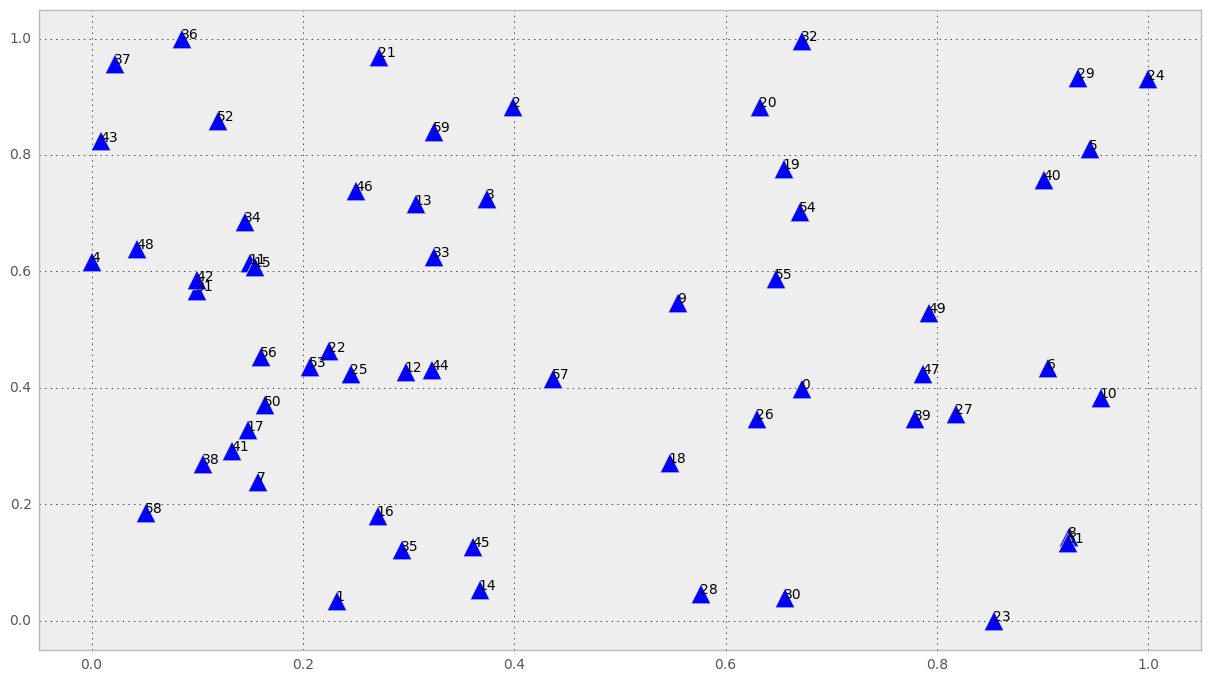
\includegraphics[width=.9\columnwidth]{rnd_example}
	\caption[random]{Esempio di istanza con layout random.}
	\label{fig:rnd}
\end{figure}

\begin{figure}[H]
	\centering
	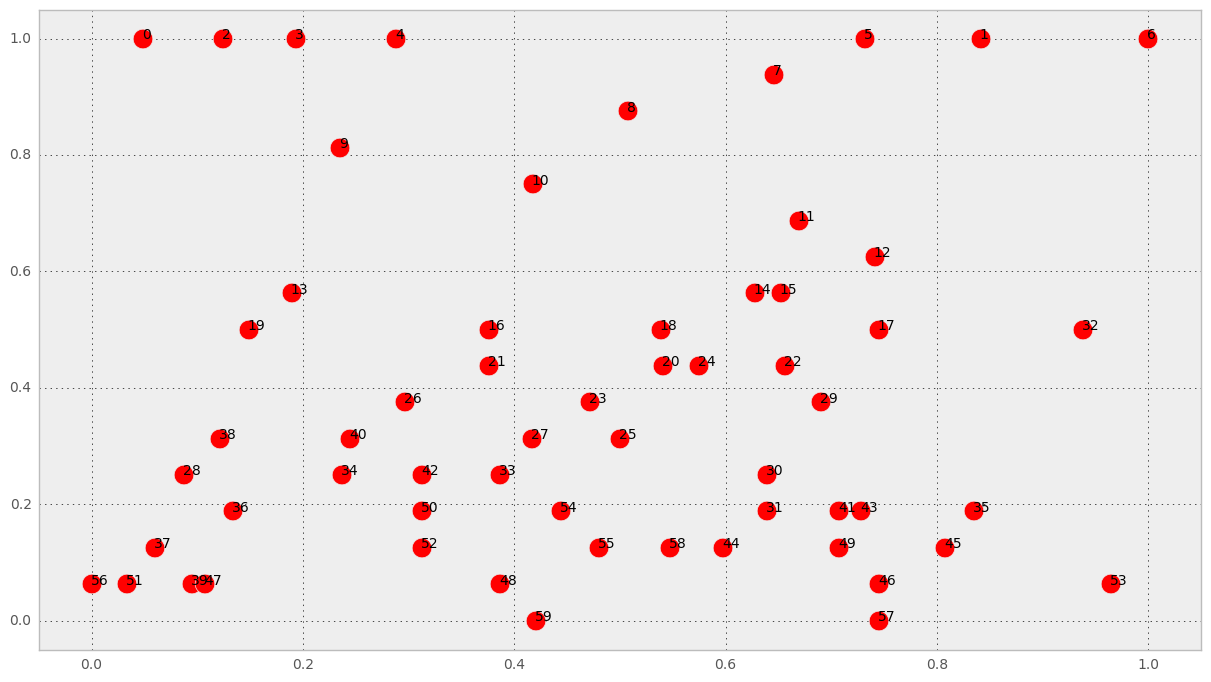
\includegraphics[width=.9\columnwidth]{cls_example}
	\caption[clustered]{Esempio di istanza con layout clustered.}
	\label{fig:cls}
\end{figure}

\subsection{Metodologia e Parametri}

Gli esperimenti consistono nell'utilizzare le tecniche descritte in Sezione \ref{sec:cplex} e \ref{sec:eur} per risolvere il TSP, sui dataset generati. Per ogni dataset, ogni risolutore viene eseguito 5 volte, e vengono salvate le medie e le standard deviation dei tempi di esecuzione e dei costi delle soluzioni ottime trovate. Gli esperimenti sono stati svolti su macchine con processore Intel Core i5-2500 da 3.30 GHz. 

Per \textsc{pso} e' stata utilizzata una popolazione di 2.000 individui, 500 iterazioni, $\alpha = 0.75$, $\beta=0.1$ (i parametri sono stati scelti empiricamente, senza un estensivo procedimento di ottimizzazione).

\subsection{Risultati}
In questa sezione vengon riportati i risultati degli esperimenti. Se non diversamente riportato, i valori nei grafici sono inizialmente mediati sulle diverse esecuzioni sul singolo dataset, e sono poi mediati sui diversi dataset.

In Figura \ref{fig:uno} e' riportato il tempo di esecuzione in scala logaritmica per le diverse dimensioni dei dataset, diviso per metodo di risoluzione e per tipo di distanza. Si puo' vedere che \textsc{cplex} confrontato con \textsc{pso} e' piu veloce per dimensioni basse del problema, mentre diventa piu' lento all'aumentare del numero di nodi. Questo e' dovuto al fatto che \textsc{cplex} ha tempo di esecuzione esponenziale nella dimensionalita' del problema, ma mostra che per problemi piccoli e' una valida opzione. Dal grafico si puo' inoltre notare che \textsc{pso} e' relativamente lento gia' a dimensioni basse. Infatti tale metaeuristica ha una rappresentazione del problema non banale e quindi richiede dell'overhead iniziale per l'inizializzazione della popolazione e il successivo aggiornamento delle velocita'. Inoltre il numero di valutazioni di funzione utilizzate e' molto alto (2.000 $\times$ 500 = 1.000.000), e non e' presente un criterio di fermata (il che significa che vengono effettuate tutte le valutazioni di funzione ad ogni esecuzione).
\begin{figure}[htpb]
	\centering
	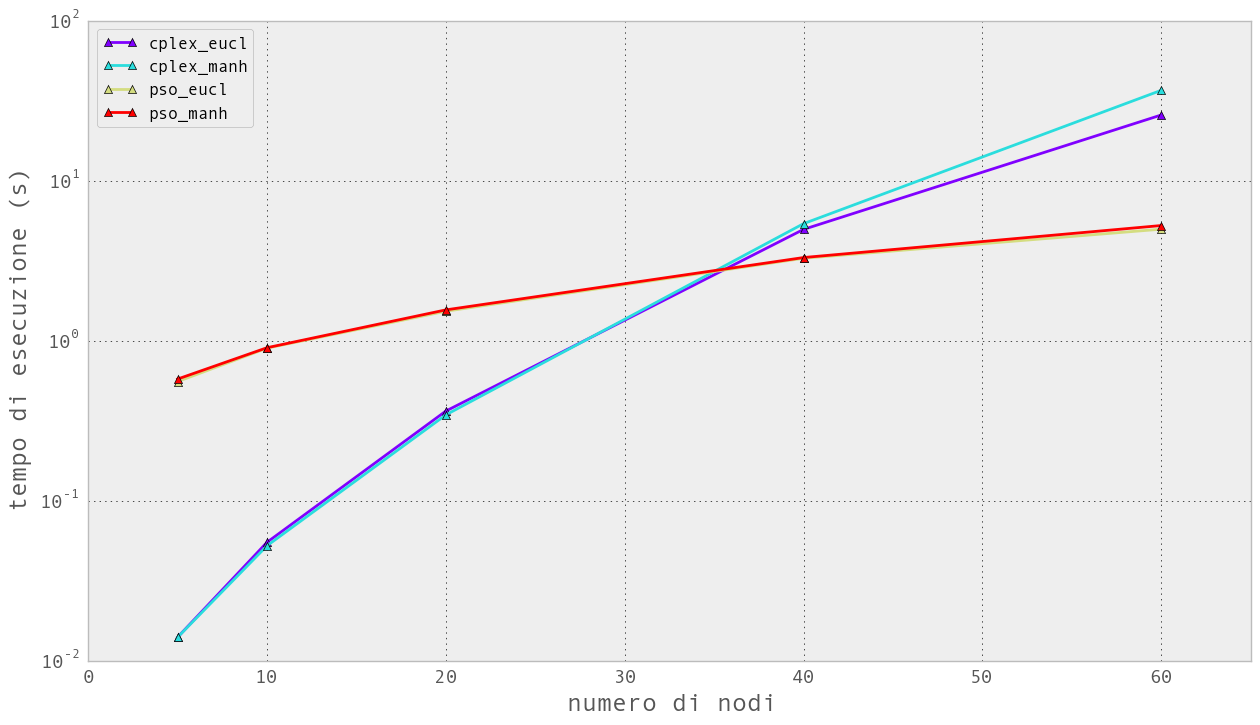
\includegraphics[width=.9\columnwidth]{uno}
	\caption[]{Tempi di esecuzione medi per le diverse dimensioni, divisi per metodo e tipo di distanza.}
	\label{fig:uno}
\end{figure}

In Figura \ref{fig:due} e' riportato il tempo di esecuzione in scala logaritmica per le diverse dimensioni dei dataset, diviso per metodo di risoluzione e per criterio di disposizione dei punti. COMPLETA QUI VEDI CHE VIEN FUORI

\begin{figure}[H]
	\centering
	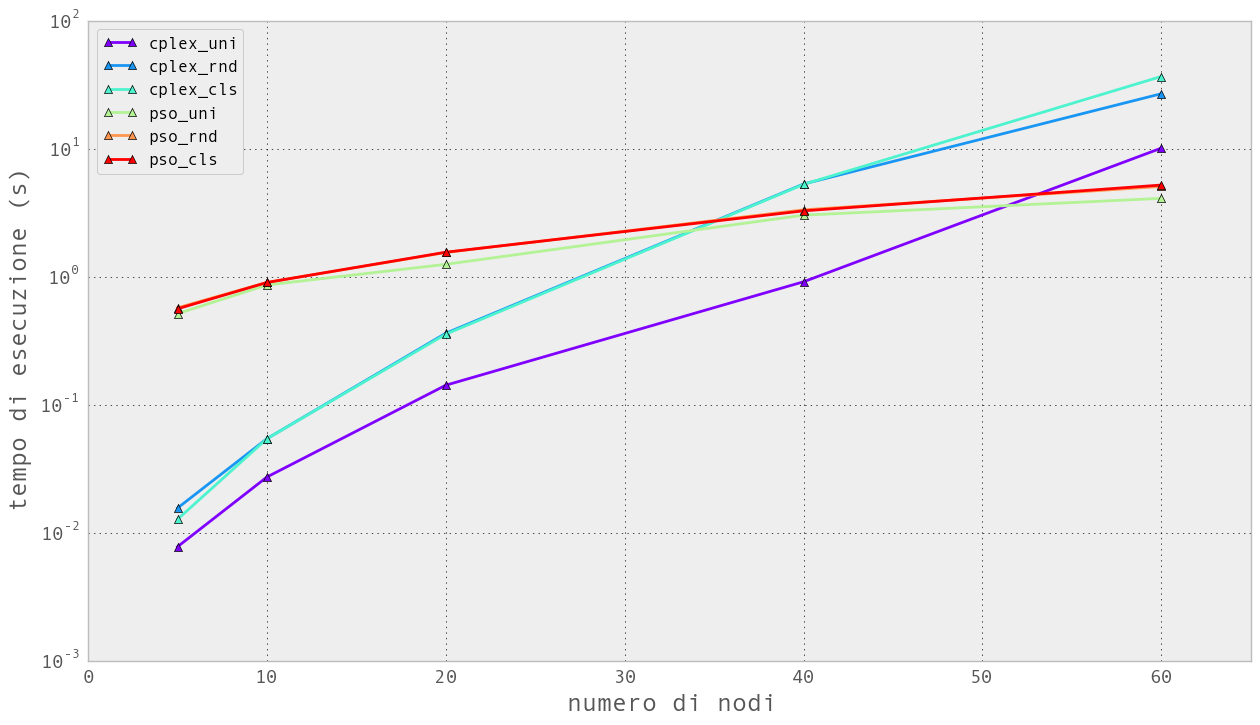
\includegraphics[width=.9\columnwidth]{due}
	\caption[]{Tempi di esecuzione medi per le diverse dimensioni, divisi per metodo e criterio di disposizione dei punti del problema. }
	\label{fig:due}
\end{figure}

In Figura \ref{fig:tre} e' riportato l'errore medio della soluzione trovata da \textsc{pso}, in percentuale, sul costo della soluzione ottima. Viene inoltre riportato lo scarto quadratico medio di tale errore. Si puo' vedere che \textsc{pso} e' relativamente efficace a basse dimensioni, questo e' dovuto al fatto che con 1.000.000 valutazioni di funzione e' possibile esplorare buona parte dello spazio delle soluzioni su dataset ridotti. La metaeuristica diventa meno precisa a partire da 20 nodi, fino ad arrivare ad un errore medio del \textasciitilde 43\% con 60 nodi.

\begin{figure}[htpb]
	\centering
	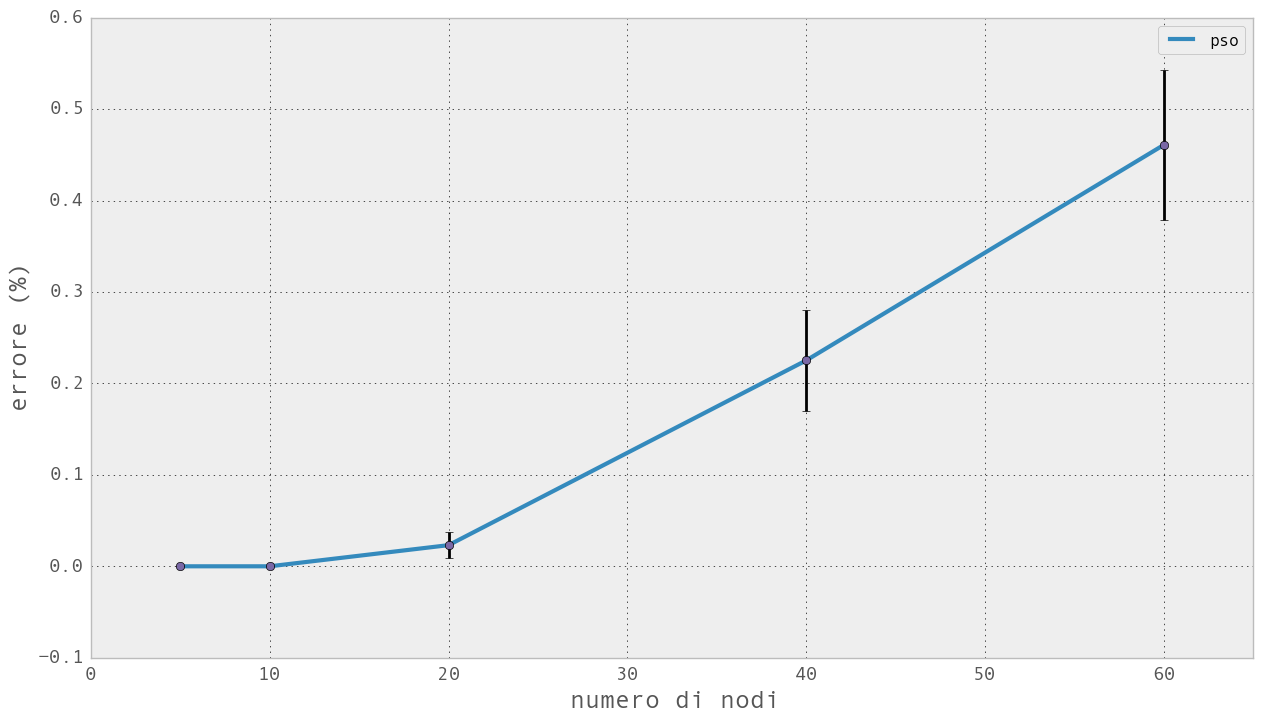
\includegraphics[width=.9\columnwidth]{tre}
	\caption[]{Media e scarto quadratico medio della percentuale di errore di \textsc{pso} rispetto alla soluzione ottima.}
	\label{fig:tre}
\end{figure}

In Figura \ref{fig:quattro} e' riportato il miglioramento della miglior soluzione trovata da \textsc{pso} (in termini di funzione obiettivo) durante l'ottimizzazione. Per ottenere delle medie significative, il valore riportato e' calcolato come la percentuale dell'errore della soluzione corrente (all'iterazione $i$-esima) rispetto all'ottimo trovato da \textsc{cplex}. Si puo' vedere che per dimensionalita' basse \textsc{pso} converge in fretta alla miglior soluzione (che generalmente e' ottima). Al crescere della dimensione del problema, la convergenza diventa piu' lenta, ma la discesa piu' veloce (anche perche' l'errore di partenza e' piu' alto). Infatti, per esempio per 40 nodi, si passa da un errore iniziale sull'ottimo di piu del 180\%, e si arriva alla fine dell'ottimizzazione ad un errore di meno del 20\%. Questo e' significativo, mostra che l'ottimizzazione funziona, ma che non e' in grado di arrivare ad una soluzione buona.

\begin{figure}[H]
	\centering
	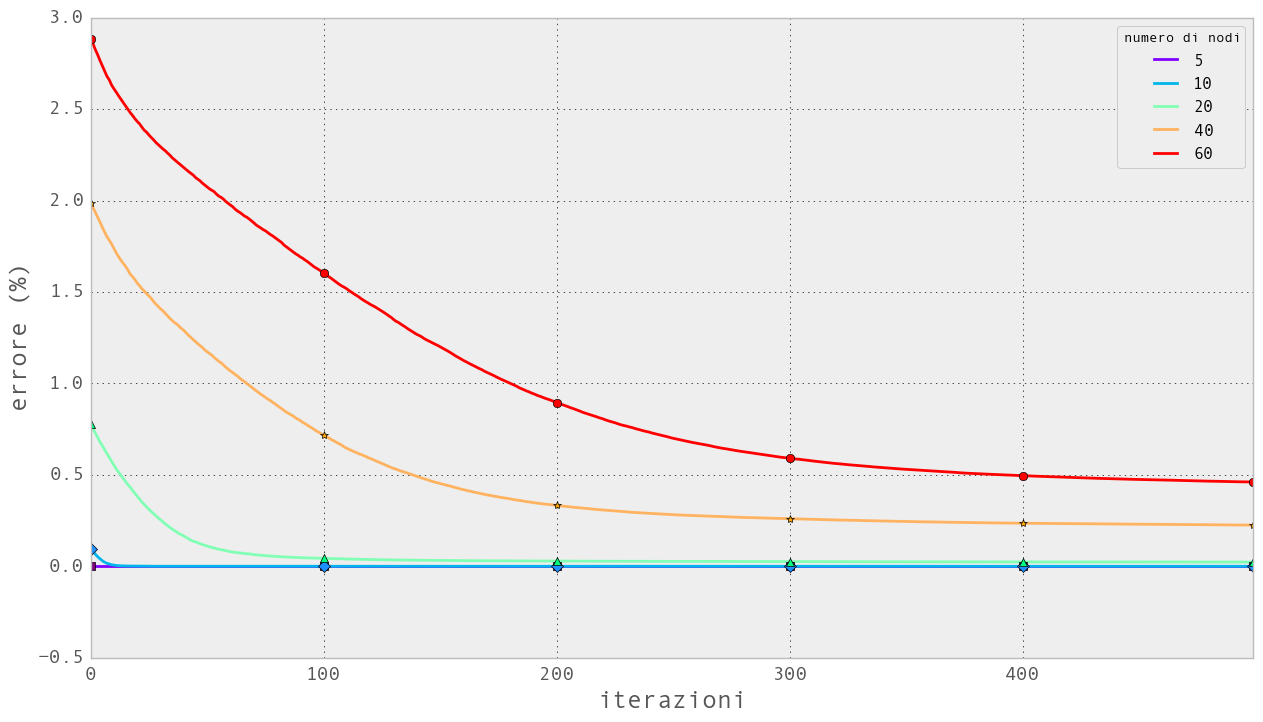
\includegraphics[width=.9\columnwidth]{quattro}
	\caption[]{Percentuali di errore della miglior soluzione trovata finora rispetto all'ottimo, durante le iterazioni di \textsc{pso}, divise per numero di nodi.}
	\label{fig:quattro}
\end{figure}

Potrebbe essere interessante vedere in PERCENTUALE RUSPE quanti degli archi usati da pso sono parte dell'ottimo. 
\section{Conclusioni}\label{sec:conclusioni}

Durante l'implementazione di questa versione di \textsc{pso} ho avuto modo di notare alcuni difetti. Infatti sono dell'opinione che in questo schema manchi una componente che permetta di esplorare la \textit{neighborhood} senza necessariamente muoversi verso una delle soluzioni gia' visitate. Infatti con tale mancanza, una volta generate gli individui iniziali, tutte le modifiche alle velocita' ``muovono'' gli individui verso uno degli altri, e non c'e alcuna garanzia che l'ottimo stia in questi percorsi. Infatti i risultati mostrano che \textsc{pso} non riesce a performare in maniera discreta oltre i 20 nodi, commettendo errori notevoli.
 
Nonostante cio', ho potuto vedere che \textsc{pso} e' molto piu' veloce di un metodo esatto quale \textsc{cplex}. In particolare, con l'aggiunta di un criterio di terminazione (e.g.: terminare l'ottimizzazione se la miglior soluzione trovata non migliora per $50$ iterazioni), la metaeuristica terminerebbe rapidamente per dimensionalita' basse, con risultati discreti. Infatti \textsc{cplex} diventa estremamente lento al crescere del numero dei nodi, il che lo rende inutilizzabili in contesti reali.
%----------------------------------------------------------------------------------------
%	BIBLIOGRAPHY
%----------------------------------------------------------------------------------------

\renewcommand{\refname}{\spacedlowsmallcaps{References}} % For modifying the bibliography heading

\bibliographystyle{unsrt}

\bibliography{bibliography.bib} % The file containing the bibliography

%----------------------------------------------------------------------------------------

\end{document}
